\chapter{Zusammenfassung \& Ausblick}
\label{chap:summ_futu}
\label{chap:summary}
\label{chap:future_work}

\section{Zusammenfassung}
\label{sec:summary}

In dieser Arbeit wurde eine lizenzfreie Produktdatenbank konzipiert und 
entwickelt um ähnliche oder darauf aufbauende Arbeiten zu vereinfachen. Mit 
Hilfe einer Webanwendung kann diese Datenbank von den Nutzer*innen bearbeitet 
und erweitert werden. Der Fokus liegt dabei auf der automatisierten Bestimmung 
der Veganität mit Hilfe der Zutatenlisten, Produktanfragen an die 
Hersteller*innen und Nutzer*innenkommentare.
Im Supermarkt können diese Informationen mit Hilfe einer mobilen Anwendung zu 
einer Kaufentscheidung genutzt werden.
Zudem kann \name durch die Internationalisierung in anderen Ländern schnell und 
einfach lokalisiert werden.\\
Die genannten Punkte sind zur Abgrenzung von anderen Arbeiten erneut in
Tabelle~\ref{table:summary}
dargestellt, wobei bei \name alle Kriterien, die in Kapitel~\ref{chap:related_work}
genannt wurden, umgesetzt wurden, was durch das grüne 
Häkchen (\cmark) symbolisiert wird.

\begin{table}[htb]
\begin{adjustwidth}{-1in}{-1in}% adjust the L and R margins by 1 inch
\centering
\rowcolors{2}{gray!25}{white}
\begin{tabular}{rccccc}
	 &
	\rot{\textbf{barcoo}} &
	\rot{\textbf{das-ist-drin}} &
	\rot{\textbf{EuLa-Armband}} &
	\rot{\textbf{MENSSANA}} &
	\rot{\textbf{\name}}\\
	\hline

	\textbf{Veganität} &
	(\cmark) &
	(\cmark) &
	\xmark &
	(\cmark) &
	\cmark\\
	
	\textbf{Plattformunabhängig} &
	\cmark &
	\cmark &
	\xmark &
	\cmark & 
	\cmark\\
	
	\textbf{Lizenzfreiheit} &
	\xmark &
	\xmark &
	\xmark &
	\xmark &
	\cmark\\
	
	\textbf{Zugang} &
	\cmark &
	\cmark &
	\xmark &
	\cmark &
	\cmark\\
	
	\textbf{Nutzer*innenbasiert} &
	\xmark &
	\cmark &
	\xmark &
	(\cmark) &
	\cmark\\

	\textbf{Lokalisierung} &
	\xmark &
	\xmark &
	\cmark &
	\cmark &
	\cmark\\

\end{tabular}
\caption{Gegenüberstellung von \name mit den verwandten Arbeiten anhand 
verschiedener Kriterien}
\label{table:summary}
\end{adjustwidth}
\end{table}
\medskip % adds some space after the table

\name ist online verfügbar und kann durch eine Lizenz, die die
Veränderung erlaubt (vgl. Abschnitt~\ref{sec:implementation:licenses}),
modifiziert und erweitert werden.
Eine technische Dokumentation, die sich auf der beiliegenden CD befindet, 
beschreibt die Installation von \name auf einem Server.

\section{Ausblick}
\label{sec:future_work}

Im Folgenden werden Möglichkeiten beschrieben, wie diese Arbeit
in Zukunft verfeinert und erweitert werden kann.
Da die Arbeit dank der Lizenzen (vgl. Abschnitt~\ref{sec:implementation:licenses})
verändert werden kann, sind diese Erweiterungen
rechtlich und technisch möglich.

\subsection{Computerlinguistische Verbesserungen}
\label{sec:future_work:coli}

Der in Abschnitt~\ref{sec:implementation:ingredients} beschriebene Parser könnte 
mit
Hilfe von computerlinguistischen Methoden verbessert werden.

Probleme gibt es bei diesem nämlich z.\,B. bei Zutaten wie
"`Mono- und Diglyceride"', da diese nicht in "`Monoglyceride"' und
"`Diglyceride"' aufgeteilt werden.
Ebenso können nähere
Informationen über eine Zutat verloren gehen, dies ist z.\,B. bei "`Pflanzenöl
ungehärtet (Kokos)"' der Fall, da hier "`Kokos"' vom Rest getrennt
wird. Insbesondere tritt dieses Problem bei Allergenen oder Spuren
auf, bspw. bei "`Lecithine (Soja)"', wobei hier Soja nur eine der
benutzten Lecithine sein kann, durch die Deklarierung von Allergenen aber
hervorgehoben werden muss \citeweb{bmelv:allergene}.
Diese Probleme könnten mit einer eigenen Zutatengrammatik oder einer Baumgenerierung gelöst
werden, z.\,B. im Rahmen einer Computerlinguistik-Arbeit.\\
Ebenso könnten die Zutatensynonyme um Fremdsprachen erweitert werden,
sodass auch das Parsen von Medikamenten oder Kosmetikartikeln, die
üblicherweise in englischer Sprache verfasst sind, leichter fällt \citeweb{bvl:inci}.
Dabei könnte bei allen Zutaten auch jeweils der Singular bzw. Plural
mit gespeichert werden.\\
Mit weitreichenden Verbesserungen könnte auch -- sofern ein Mailserver
konfiguriert ist -- eine eingehende E-Mail geparst werden und
automatisch einsortiert werden.

\subsection{Veganitätsbestimmung}
\label{sec:future_work:veganity}

Eine weitere Verbesserung wäre der Einbau einer Logik, mit der die
Veganität eines Produktes anhand anderer Angaben bestimmt werden
kann, wie in Abbildung~\ref{img:veganity_logic} dargestellt ist.

\begin{figure}[ht]
	\begin{adjustwidth}{-1in}{-1in}
	\centering
	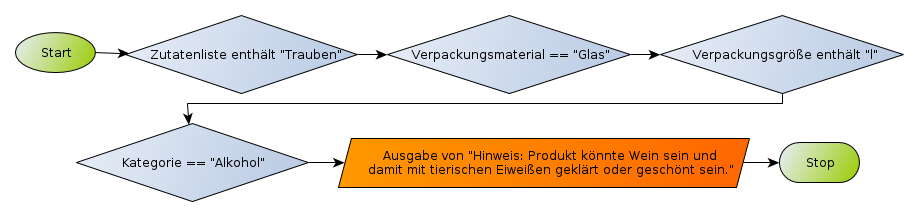
\includegraphics[scale=0.5]{misc/veganity_logic.png}
	\caption{Flowchart zur Bestimmung der Veganität aus
	den Produktangaben}
	\label{img:veganity_logic}
	\end{adjustwidth}
\end{figure}

In diesem Beispiel wird formal eine Flasche Wein durch Entscheidungen
beschrieben, wobei im Erfolgsfall ein Hinweis angezeigt wird, dass
dieses Produkt unvegan sein könnte.
Diese Logik könnte spielerisch zusammengesetzt werden (wie es bei dem
visuellen Programmeditor "`Blockly"' der Fall ist \citeweb{google:blockly})
oder als Logik in einer XML-Datei angegeben werden und
durch ein*e Administrator*in hochgeladen werden.\\
Auf dieser Logik aufbauend könnte auch eine Produktanfrage besser
generiert werden, indem direkt nach den Regeln dieser Logik Fragen
gestellt werden.

\subsection{OCR und -Reader}
\label{sec:future_work:ocr}

Um die Zutatenlisten nicht mühsam von Hand eintippen zu müssen,
würde sich zusammen mit der App \ac{OCR} (auch Texterkennung oder Optische Zeichenerkennung
genannt) anbieten, welches eine automatisierte Texterkennung innerhalb von
Bildern möglich macht.\\
In dem Beispiel in Abbildung~\ref{img:ocr} wurde die Aufschrift auf
der Verpackung mit Hilfe der Android-App "`OCR Test"' komplett
erkannt.

\begin{figure}[ht]
	\centering
	\frame{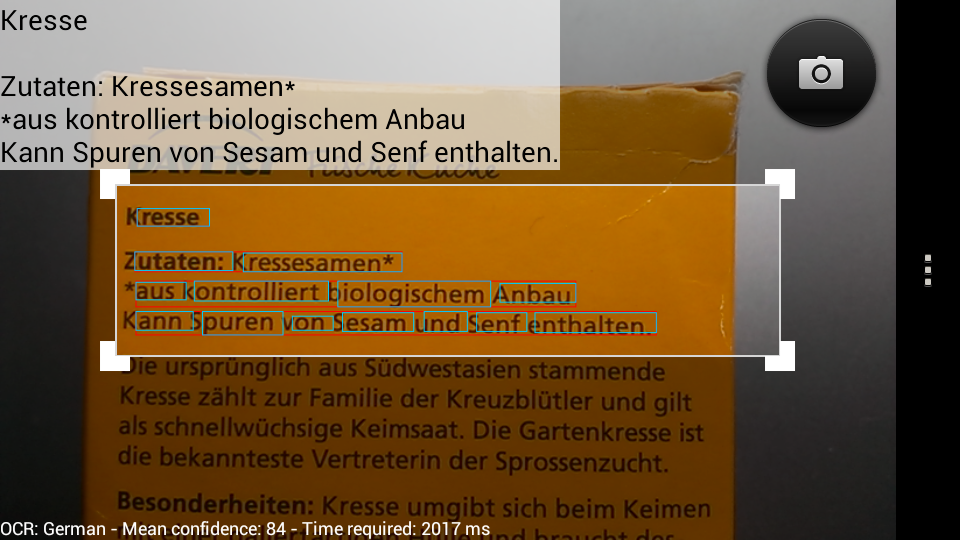
\includegraphics[scale=0.4]{pics/ocr-kresse.png}}
	\caption{OCR am Beispiel einer Kresse-Verpackung}
	\label{img:ocr}
\end{figure}

Da dies nicht immer der Fall ist, weil die aufgenommenen
Gegenstände rund sein oder die Umgebung schlecht beleuchtet sein
könnte, könnte auf Grundlage der erkannten Buchstaben und mit Hilfe
der Levenshtein-Distanz, mit der Textunterschiede gemessen werden
können und den vorhandenen Produkt- bzw. Zutatendaten in der Datenbank
diese Arbeit erweitert werden \cite{dlph10, shs11, kac12}.
